% Chapter Template

% Main chapter title
%\chapter[toc version]{doc version}
\chapter{Background}

% Short version of the title for the header
%\chaptermark{version for header}

% Chapter Label
% For referencing this chapter elsewhere, use \ref{ChapterTemplate}
\label{ChapterBackground}

% Write text in here
% Use \subsection and \subsubsection to organize text

The main focus of this chapter is to provide the reader with the necessary background to understand the context and technical 
foundations of this project. The goal of the system is to automatically evaluate network topologies by validating 
configurations and executing tests across various devices within a virtual network.

Achieving this requires the integration of multiple technologies, as the system must support a wide range of features to 
deliver a fully automated, end-to-end solution. Key concerns include not only functionality but also scalability, since 
multiple students may interact with the platform concurrently, each requiring an isolated working environment.

To support these requirements, this chapter introduces core concepts and tools such as virtualization, network automation, 
web frameworks and task processing. These components form the foundation upon which the system is built.


\section{Virtualization}
Virtualization is the process of creating a virtual version of physical resources, such as routers, switches, or even
entire computers. In the context of this project, it is used to create virtual machines to provide students with a 
work environment and virtual networks, comprised of various types of virtualized devices. This approach enhances scalability 
and reduces costs, as it allows multiple virtual machines to be run on a single physical machine.

Virtualization can be categorized into \textbf{emulation} and \textbf{simulation}. 

\begin{itemize}
  \item Emulation is the process of creating a virtual version of a physical device in software, replicating its 
  behavior exactly—including any bugs and limitations. This is useful for various things like testing software on 
  different platforms, running legacy software on modern hardware and even running potentially harmful software in a safe 
  isolated environment.
  Emulation will be used to provide students with a work environment to test their network configurations,
  as well as to emulate certain network devices.
  \item Simulation models the behaviour of a device, without replicating the underlying hardware or software.
  This results in a simpler less resource intensive model, though it may not fully capture the real device's behavior.
  Simulation will be used to simulate the behaviour of certain, simpler and generic, network devices.

\end{itemize}


\section{GNS3}
\ac{gns3} is an open-source graphical network emulator software that allows the user to create complex network topologies 
and interact with the various devices in it. It is widely used for educational purposes and is often used in preparation 
for professional network certifications like the Cisco Certified Network Associate (CCNA).

\ac{gns3} employs a simple drag and drop interface to allow users to add new devices, make links between them 
and even add textual annotations. The software allows users to interact with the devices by way of a console or even a GUI
if the device supports it. The software also allows users to export their topologies to be shared with others, which can
be useful for teachers to provide students with a pre-configured topology to work on.

Additionally, the software supports packet capturing which is essential for students to develop their debugging and 
troubleshoting skills. Finally it can also be interacted with via a\ac{rest}\ac{api} which is of particular interest
for this project.

\subsection{Architecture}
The software can be employed in a variety of ways due to its architecture \cite{GNS3Architecture} that separates the user 
interfaces that it offers, namely the locally installed gns3-gui as well as the browser accessible gns3-web, from the 
gns3-server that runs the emulations and the controller who orchestrates everything.

\subsubsection{Controller}
The controller is integrated in the gns3-server project and is responsible for communicating with all the other components 
of the software. The controller is a singleton, meaning there should only be one instance of it running at any given time, 
and it does not support concurrent requests. It is able to control multiple compute instances if so desired, each capable 
of hosting one or more emulator instances, varying depending on their complexity. The controller also exposes the 
\ac{rest}\ac{api} allowing the ability to interact with the software programatically. All communication is done over
\ac{http} in\ac{json} format and there is support for basic\ac{http} authentication as well as notifications via websockets.

\subsubsection{Compute}
The compute is also integrated in the gns3-server project and controls the various emulators required to run the nodes 
in the topology.
The list of currently supported emulators is:

\begin{itemize}
    \item \textbf{Dynamips} - Used to emulate Cisco routers and basic switching.
    \item \textbf{\ac{iou}} - Used to emulate Cisco\ac{ios} devices.
    \item \textbf{\ac{qemu}} - Used to emulate a wide variety of devices.
    \item \textbf{\ac{vpcs}} - A basic program meant to simulate a basic PC.
    \item \textbf{VMware/VirtualBox} - Used to run virtual machines with nested virtualization support.
    \item \textbf{Docker} - Used to run docker containers.
  \end{itemize}

\subsubsection{GUI}
The GUI is composed of two separate but with mostly identical functionality, namely the gns3-gui and the gns3-web projects.
The gns3-gui project is a desktop application that is used to to interact with a local or remote gns3-server instance. It 
is written in Python and uses the Qt framework for the graphical interface. The gns3-web is a web application that is 
accessed via a web browser it is still in a beta stage but is already capable enough to be used as a substitute for the 
gns3-gui.

\begin{figure}
    \centering
      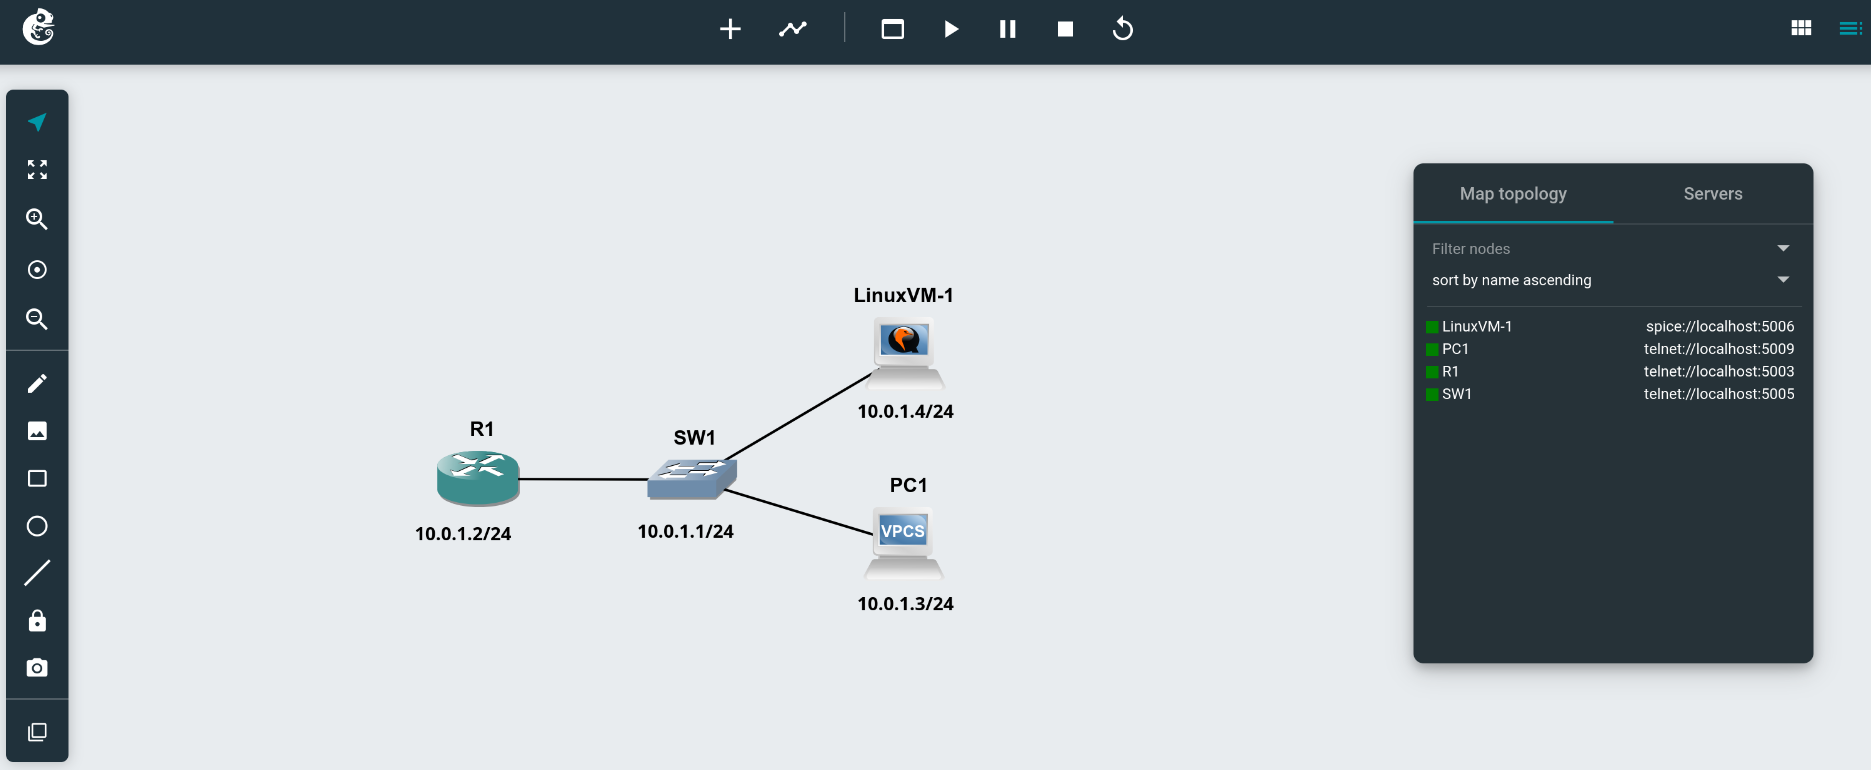
\includegraphics[width=.95\linewidth]
        {Background/gns3-web.png}
    \caption{A simple network topology example in the GNS3 Web UI}
	\hfill
\end{figure}

\section{Linux}
Linux is a core component of this project, as it is the kernel of all operating systems used to host all the services provided.

\begin{itemize}
  \item \textbf{Containerized Web Application} - The web application runs inside an LXC container on Proxmox. Since LXC 
  containers share the host kernel, the containerized web application benefits from efficient resource usage while maintaining 
  isolation from the host system.
  \item \textbf{Virtual Machines hosting GNS3} Proxmox also hosts virtual machines running Linux-based Ubuntu GNS3 servers. 
  These VMs provide students with isolated environments to configure and test network topologies, benefiting from the 
  flexibility of full virtualization through KVM, giving them the ability to virtualize any type of network device.
  Students only interact with these \ac{vm}s via the GNS3 web Interface. Students interact with these VMs using a browser, 
  accessing the gns3-server instance running on them. Thus the students never have to interact with the underlying 
  operating system, and so these machines do not require a desktop environment, which helps freeing up resources leading to
  better scalability.
  \item \textbf{\ac{pve}} - Proxmox is a Linux-based open-source platform for enterprise-level virtualization. It is based
  on the Debian Linux distribution.
\end{itemize}


\section{Proxmox Virtual Environment} 
\ac{pve} is an open-source platform designed for enterprise-level virtualization \cite{proxmox2025}. It is based on the Debian
distribution of Linux and provides a web-based interface for managing virtual machines and containers. It is widely used
in data centers and cloud environments, as it provides a scalable and reliable solution for virtualization.

\ac{pve} bundles several core services that can be interacted with via shell commands, a web interface or even by using
the \ac{pve}\ac{rest}\ac{api}.
These allow the user to interact with every service provided by \ac{pve}, in a plethora of ways, depending on the user's
needs, skills and preferences. The web interface is the most user-friendly way to interact with the platform, as it
provides a graphical interface for managing the cluster. The shell commands provide a more direct way to interact with the
platform, allowing for more complex operations to be performed and opening the doors to scripting and automation. Finally,
the \ac{pve}\ac{rest}\ac{api} allows for programmatic interaction with the platform, enabling users to create custom
applications that can interact with the platform.


\subsection{Virtualization Technologies}
\ac{pve} supports the the deployment and management of two distinct types of virtualization, namely, \ac{kvm}- 
based\ac{vm}s and\ac{lxc}-based containers.

Users can interact with these virtualized environments via NoVNC, a simple web-based VNC client or SPICE which is a more
feature-rich protocol that provides better performance and more features than VNC.
Both of these protocols support the use of a console-based interface, aswell as a full desktop graphical interface.


\subsubsection{\ac{kvm}}
\ac{kvm} is a virtualization solution provided by the Linux kernel. It leverages the hardware virtualization extensions 
of modern processors to provide a full virtualization experience at near-native speeds. Supports a wide range of guest 
operating systems making it a good choice for general purpose virtualization.

In \ac{pve},\ac{kvm} is used as the core component for running virtual machines and is used alongside \ac{qemu}.

\subsubsection{\ac{lxc}}
Containerization is an operating system-level virtualization method that packages an application and its dependencies
together into an isolated environment. Contrary to tradional\ac{vm}s, containers dont emulate hardware or require a 
guest operating system relying instead on the host's kernel. This approach leads to a faster and more lightweight 
virtualization solution, as they consume less memory and cpu resources.

\ac{lxc} creates full system containers, capable of simulating a complete Linux distribution providing users with an 
environment that behaves like a traditional\ac{vm} but with the speed and efficiency of a container. \ac{lxc} start 
much faster than \ac{vm}s making them ideal for scenarios requiring rapid deployment and/or scaling.

However, it's important to note that while containers offer a degree of isolation, they do not provide the same level of
security as\ac{vm}s. This means that while they may not always be a suitable replacement for\ac{vm}s.

\section{Python}
Python is a high-level, interpreted programming language renowned for its readability and versatility. It supports 
multiple programming paradigms, including procedural, object-oriented, and functional programming, making it suitable 
for a wide array of applications.
In the context of this project, Python serves as the primary programming language as its extensive standard library 
and supportive community contribute to efficient development and maintenance of the project's codebase.

\subsection{WSGI}
The\ac{wsgi} is a pivotal standard for Python web application deployment, defining a consistent interface between web 
servers and Python applications or frameworks.

Prior to \ac{wsgi}'s introduction, Python web frameworks were typically written against various server-specific APIs such as 
CGI, FastCGI, or mod\_python. This diversity led to compatibility issues, limiting developers' choices of web servers and 
frameworks, as not all frameworks supported all web servers and vice-versa. To address this fragmentation, \ac{wsgi} was 
created as a standardized interface, promoting portability and flexibility in deploying Python web applications. 

\ac{wsgi} serves as a bridge, enabling web servers to communicate with Python applications. It specifies a simple and universal 
interface for web servers to forward requests to Python applications and for those applications to return responses. 
This standardization allows developers to choose from a variety of web servers and Python frameworks without compatibility 
concerns\cite{pep333}.

Introduced in 2003 as PEP 333, \ac{wsgi} was later updated to PEP 3333 in 2010 to accommodate Python 3. These specifications 
outline how web servers and Python applications should interact, ensuring a consistent and reliable deployment environment 
across different platforms.

The \ac{wsgi} standard consists of two main components:
\begin{itemize}
  \item \textbf{Server/Gateway Side} - Responsible for receiving\ac{http} requests from clients and passing them to the 
  Python application. Then receives the response from the application and forwards it to the client. 
  \item \textbf{Application} - The Python application that processes requests and returns responses.
\end{itemize}

Additionally \ac{wsgi} has support for middleware components. \ac{wsgi} middleware is a Python callable that wraps another 
\ac{wsgi} application to observe or modify its behavior. Middleware can perform various functions, including request 
preprocessing, response postprocessing, session management, and security checks. This modularity allows developers to 
add functionality to their applications in a reusable and maintainable manner.

The separation defined by \ac{wsgi} allows for flexibility and scalability in deploying Python web applications.

During development, Python \ac{wsgi} applications often use built-in servers provided by frameworks like Flask. 
However, these servers typically aren't fully featured and aren't suitable for production environments. In production, WSGI 
servers act as intermediaries between web servers (e.g., NGINX or Apache) and Python applications, handling incoming requests 
and serving responses efficiently.

\subsubsection{Flask}
Flask is a web application micro framework written in Python, adhering to the \ac{wsgi} standard, designed to 
facilitate the development of web applications by providing essential tools and features. Classified as a microframework, 
Flask does not require particular tools or libraries, instead choosing to focus on simplicity and extensibility\cite{flask2025}.

Initially, Flask served as the backbone for the entire project, providing the necessary infrastructure to handle HTTP 
requests, render templates, and manage application routing. Its flexibility and minimalistic approach allow for the 
integration of various extensions and libraries as needed, ensuring the application remains lightweight yet functional. 
Flask's comprehensive documentation and supportive community further enhance its suitability by the creation and support
of community-driven extensions speeding up development and reducing the need to reinvent the wheel.

An example of how easy it is to develop a basic web application with flask is provided in the following small 
piece of code.

\begin{algorithm}
  \caption{Flask Hello World}\label{flask-hello-world}
  \begin{algorithmic}[1]
    \State \textbf{from} flask \textbf{import} Flask
    \State \textbf{app} = Flask(\_\_name\_\_)
    \State
    \State \textbf{@app.route('/')}
    \State \textbf{def} hello\_world():
    \State \hspace{1em} \textbf{return} 'Hello, World!'
    \State
    \State \textbf{if} \_\_name\_\_ == '\_\_main\_\_':
    \State \hspace{1em} app.run()
  \end{algorithmic}
\end{algorithm}

While Flask remained suitable for early development, emerging requirements—particularly those involving asynchronous 
processing and more scalable I/O operations—eventually led to an architectural shift, in part due to Flask's limited async 
support. This transition is discussed in detail in the following sections, where the adoption of \ac{asgi}-compatible 
frameworks and asynchronous tools is explored.

\subsection{Celery}
Celery is an open source distributed task queue focused on real-time processing but also offers support for task scheduling.
It is implemented in Python, but the underlying protocol can be implemented in any language. Celery requires a message broker 
to function, such as Redis or RabbitMQ, which are responsible for queuing and distributing tasks from producers (clients) to 
consumers (workers).

A Celery client running on a given machine will have allocated a set amount of workers to work on tasks. Workers are 
independent processes that listen to the broker and execute incoming tasks concurrently. Tasks are Python functions that 
are decorated with provided Celery decorators such as \texttt{@app.task}, causing them to be registered as Celery tasks 
within the Celery application.

\begin{algorithm}
  \caption{Calling a Celery Task and Getting the Result}\label{celery-call-result}
  \begin{algorithmic}[1]
    \State \textbf{from} celery \textbf{import} Celery
    \State
    \State \textbf{app} = Celery('tasks', broker='redis://localhost:6379/0', backend='redis://localhost:6379/0')
    \State
    \State \textbf{@app.task}
    \State \textbf{def} hello():
    \State \hspace{1em} \textbf{return} 'hello world'
    \State
    \State \textbf{result} = hello.delay()
    \State \textbf{print}(result.get())
  \end{algorithmic}
\end{algorithm}

To execute a task, a Celery task function must be called using the \textit{delay()} method, which will return a result object. 
This result object can be used to check the status of the task and to retrieve the result once it is available.

Celery supports horizontal scaling by design, allowing multiple worker pools to run on separate physical or virtual machines. 
This makes it especially effective for handling growing workloads—for example, processing email newsletters for an expanding 
user base.

In addition to basic task execution, Celery provides advanced features such as retry policies, task chaining, prioritization, 
and timeouts. However, these benefits come with added complexity in deployment and maintenance, especially regarding broker 
reliability, result backend persistence, and worker supervision.

Furthermore, Celery clients and workers introduce a non-negligible overhead in terms of CPU and memory usage, even when 
idle, as they must maintain persistent connections to the broker and periodically perform health checks or heartbeats. 
This can be a concern in resource-constrained environments or during development.This overhead became especially evident 
during early integration tests.

As the project evolved, it became increasingly clear that Celery's benefits did not outweigh its resource and 
architectural costs for the current use case. This realization prompted an exploration of more lightweight asynchronous 
alternatives, eventually culminating in a migration to FastAPI—an \ac{asgi}-compliant framework with native async capabilities 
and simpler concurrency management.

\subsection{Asyncio}

Asyncio is Python library for writing concurrent code. It provides a foundation for asynchronous programming by enabling 
the creation and management of event loops, coroutines, and asynchronous tasks.

An \textit{event loop} is a central component of asynchronous programming—it continuously runs in the background, managing 
the execution of asynchronous tasks. When a task reaches a point where it would normally block (e.g., waiting for a network 
response), it yields control back to the event loop, which can then continue running other ready tasks. This model of 
cooperative multitasking contrasts with traditional multithreading or multiprocessing, as it operates in a single thread 
and does not require locking or context switching between OS threads.

A \textit{coroutine} is a special kind of function defined with \texttt{async def}. When called, it does not run immediately, 
but instead returns a coroutine object. This object can be scheduled by the event loop, and when awaited, it runs until it 
hits a pause point (e.g., another \texttt{await})—at which point it yields control back to the event loop, allowing other 
coroutines to execute.

This approach is particularly well-suited for I/O-bound operations—such as network communication, file access, or database 
queries—where tasks spend a significant amount of time waiting for external operations that are outside of our control to 
complete. Rather than blocking the entire application during such waits, Asyncio allows other tasks to execute in the 
meantime, leading to more efficient resource utilization and improved throughput.

In the context of this project, \texttt{asyncio} plays a critical role. The application often performs multiple concurrent 
\ac{http} requests to interact with services like \ac{gns3} and \ac{pve}. By utilizing asynchronous functions and running 
them through the event loop, the application can efficiently manage these concurrent tasks without spawning additional 
threads or processes, thus keeping overhead low.

For example, in FastAPI, declaring an endpoint as \texttt{async def} ensures that the underlying logic is non-blocking. 
If that logic includes \texttt{asyncio}-compatible I/O operations—such as using a library for asynchronous \ac{http} calls 
then the request can proceed in a truly asynchronous manner. This allows the web server to observe massive speedups when
multiple \ac{http} calls must be made to external services.

Additionally, \texttt{asyncio} supports the orchestration of multiple tasks using constructs such as \texttt{asyncio.gather()}, 
which allows multiple coroutines to be executed concurrently and awaited collectively. This has been especially useful in 
scenarios within the project where multiple devices or services must be queried or configured simultaneously.

Overall, \texttt{asyncio} provides the concurrency model that underpins FastAPI's high performance. By embracing this model, 
the project benefits from improved responsiveness, lower latency, and better scalability—especially under workloads that 
involve heavy interaction with external services.


\subsubsection{ASGI}

\ac{asgi} is an interface specification for Python web servers and applications. It is considered a spiritual successor to 
\ac{wsgi}, designed to provide a standard interface for asynchronous communication. \ac{asgi} was developed to address the 
limitations of \ac{wsgi}, which was primarily designed for synchronous applications. Unlike \ac{wsgi}, \ac{asgi} supports 
handling multiple requests concurrently, making it suitable for modern web applications that require real-time features such 
as WebSockets, long-lived connections, background tasks or the use of Python's async features.

As development progressed, asynchronous task handling became a more central requirement, initially addressed by integrating 
Celery. However, due to its resource overhead and deployment complexity, Celery was eventually phased out. This shift 
prompted an evaluation of frameworks that offered native support for asynchronous operations.

Quart—a reimplementation of Flask compatible with the \ac{asgi} standard—was initially considered due to its high degree of 
code compatibility with Flask. It promised an easy migration path while granting access to the benefits of asynchronous 
execution. However, several critical issues emerged concerning project stability, ecosystem maturity, and extension 
compatibility.

In particular, Flask extensions that were used in the project, proved incompatible with Quart, and their Quart-specific 
replacements  were often incomplete, lacking in proper documentation,  unmaintained or even abandoned.
This lack of compatibility and maturity posed significant development challenges, as many Flask extensions were essential
for the project's functionality, and finding suitable replacements in Quart proved difficult.

As a result, adopting Quart would have required extensive reimplementation effort with limited long-term confidence in the 
ecosystem.

\subsubsection{FastAPI}

FastAPI is a modern, high-performance web framework adopting the \ac{asgi} standard. It leverages open standards, such as 
\ac{oas}, for defining path operations, parameters, and more, which in turn is based on the \ac{json} schema.
FastAPI relies entirely on Python type declarations, making it more intuitive and lowering the barrier to entry to new 
developers. This approach also simplifies the understanding and maintenance of the codebase.

Built on top of Starlette, a lightweight \ac{asgi} framework, and Pydantic, a data validation library. FastAPI combines the 
strengths of both to provide a powerful and flexible framework for building APIs with automatic data validation, 
serialization and documentation generation, all of which significantly enhance developer productivity.

Another key feature of FastAPI, being \ac{asgi}-compliant, is its built-in support for asynchronous programming, allowing 
developers to write non-blocking code using Python's \textit{async} and \textit{await} keywords. This is particularly useful 
for I/O-bound operations, such as database queries or network requests, as it allows the application to handle multiple 
requests concurrently without blocking the application which is essential in projects such as this one where multiple 
concurrent \ac{http} calls are made to interact with multiple devices and services concurrently, such as \ac{gns3} and 
\ac{pve}.

Another powerful feature of FastAPI is its dependency injection system, that is very easy to use as it is automatically
handled by the framework itselft. This allows for a clean and modular codebase, as dependencies can be easily injected into
the various components of the application. This is especially useful in larger applications, where managing dependencies
can become complex and cumbersome.
This can be of particular importance for maintainabilty and extensibility as we have already seen in the previous sections 
with Flask extensions that were already integrated into the project, and that would have to be reimplemented from scratch 
in Quart, were the project to go down that path. 

Ultimately, the project transitioned to FastAPI. While the migration to FastAPI involved a fair amount of effort, this 
was anticipated from the outset—unlike Quart, which had initially seemed easier but presented unforeseen difficulties, 
it resulted in better runtime performance, improved concurrency handling, and a cleaner overall structure, when compared 
to the previous Flask implementation with Celery integration.

This change laid the groundwork for more efficient handling of I/O-bound operations—such as network interactions with 
Proxmox or \ac{gns3}, which will be of importance in future iterations of the project while also streamlining endpoint 
development thanks to FastAPI's built-in request parsing, background task support, and integrated dependency injection system.

\subsection{Nornir}
Nornir is an open-source automation framework written in Python, designed to provide a flexible and efficient 
approach to network automation tasks\cite{nornir2025}. Unlike other automation tools that utilize customized 
pseudo-languages, Nornir leverages pure Python code, offering developers the full power and versatility of the Python 
ecosystem.

Nornir supports multi-threaded task execution, allowing operations to run parallel across multiple devices.
This capability enhances efficiency and reduces the time required enabling easy scaling to a large number of devices.

The framework provides a robust inventory management system, enabling the organization of devices into groups and the 
assignment of specific tasks to these groups. This structure facilitates targeted automation and simplifies complex 
network operations.

Finally, thanks to Nornir's architecture, it is highly extensible through its plugin system, allowing users to create 
custom plugins for inventory management, task execution, and result processing. This modularity ensures that Nornir can 
adapt to a wide range of network automation scenarios.

Nornir is particularly well-suited for tasks such as configuration management and state validation which makes it 
highly desirable in the context of this project. Its ability to handle concurrent operations will also ensure it can scale 
alongside the rest of the project.

\subsection{Requests}
The Requests\cite{requests2025} library is a popular and user-friendly\ac{http} library for Python, used to send\ac{http} 
requests to web services. It simplifies interactions with \ac{api}s by simple to use methods for the various\ac{http} verbs, 
as well as providing support for cookies, sessions, authentication, \ac{json} and exception handling for network failures and 
invalid responses.

Requests was initially used in the project to handle all\ac{http} requests to the various services, such as
\ac{gns3} and \ac{pve}. Its simplicity and ease of use made it a natural choice for the initial implementation, allowing
for quick development and testing of the various endpoints.

\begin{algorithm}
  \caption{Making a Synchronous HTTP Request Using Requests}\label{requests-basic}
  \begin{algorithmic}[1]
    \State \textbf{import} requests
    \State
    \State \textbf{url} = "https://api.example.com/data"
    \State \textbf{response} = requests.get(url)
    \State
    \If{response.status\_code == 200}
      \State \textbf{data} = response.json()
      \State \textbf{print}(data)
    \Else
      \State \textbf{print}("Request failed with status code", response.status\_code)
    \EndIf
  \end{algorithmic}
\end{algorithm}

However, as the project evolved and the need for asynchronous processing became more apparent, with Requests being a 
synchronous library only, there was a need to transition to an alternative that support asynchronous operations.

\subsection{HTTPX}

HTTPX\cite{httpx2025} is a modern \ac{http} client library for Python. HTTPX retains a similar structure to 
Requests, while providing  built-in support for asyncio.

In contrast to Requests, which blocks the current thread while waiting for a response, HTTPX enables non-blocking 
\ac{http} communication when used in asynchronous mode. This is particularly beneficial in scenarios involving multiple 
concurrent network operations, such as querying multiple \ac{gns3} devices or cloning virtual machines in \ac{pve}, 
where synchronous requests would otherwise serialize execution and lead to performance bottlenecks.

\begin{algorithm}
  \caption{Making an Asynchronous HTTP Request Using HTTPX}\label{httpx-basic}
  \begin{algorithmic}[1]
    \State \textbf{import} httpx
    \State \textbf{import} asyncio
    \State
    \State \textbf{async def} fetch():
    \State \hspace{1em} \textbf{url} = "https://api.example.com/data"
    \State \hspace{1em} \textbf{async with} httpx.AsyncClient() \textbf{as} client:
    \State \hspace{2em} response = \textbf{await} client.get(url)
    \State \hspace{2em} \textbf{if} response.status\_code == 200:
    \State \hspace{3em} \textbf{data} = response.json()
    \State \hspace{3em} \textbf{print}(data)
    \State \hspace{2em} \textbf{else}:
    \State \hspace{3em} \textbf{print}("Request failed with status code", response.status\_code)
    \State
    \State asyncio.run(fetch())
  \end{algorithmic}
\end{algorithm}

HTTPX was adopted in the project to replace Requests for both asynchronous and synchronous use cases. Thanks to its full 
support for \texttt{async} and \texttt{await}, HTTPX integrates seamlessly into the FastAPI application, allowing 
concurrent \ac{http} requests to be awaited collectively using constructs like \texttt{asyncio.gather()}. This significantly 
improved the application's throughput under concurrent workloads.

Overall, HTTPX provides a robust and flexible foundation for asynchronous networking in Python, making it an ideal 
fit for the needs of this project.

\unsure{Maybe talk about the choosen asgi server}